% Options for packages loaded elsewhere
\PassOptionsToPackage{unicode}{hyperref}
\PassOptionsToPackage{hyphens}{url}
%
\documentclass[
  english,
  man]{apa6}
\usepackage{lmodern}
\usepackage{amssymb,amsmath}
\usepackage{ifxetex,ifluatex}
\ifnum 0\ifxetex 1\fi\ifluatex 1\fi=0 % if pdftex
  \usepackage[T1]{fontenc}
  \usepackage[utf8]{inputenc}
  \usepackage{textcomp} % provide euro and other symbols
\else % if luatex or xetex
  \usepackage{unicode-math}
  \defaultfontfeatures{Scale=MatchLowercase}
  \defaultfontfeatures[\rmfamily]{Ligatures=TeX,Scale=1}
\fi
% Use upquote if available, for straight quotes in verbatim environments
\IfFileExists{upquote.sty}{\usepackage{upquote}}{}
\IfFileExists{microtype.sty}{% use microtype if available
  \usepackage[]{microtype}
  \UseMicrotypeSet[protrusion]{basicmath} % disable protrusion for tt fonts
}{}
\makeatletter
\@ifundefined{KOMAClassName}{% if non-KOMA class
  \IfFileExists{parskip.sty}{%
    \usepackage{parskip}
  }{% else
    \setlength{\parindent}{0pt}
    \setlength{\parskip}{6pt plus 2pt minus 1pt}}
}{% if KOMA class
  \KOMAoptions{parskip=half}}
\makeatother
\usepackage{xcolor}
\IfFileExists{xurl.sty}{\usepackage{xurl}}{} % add URL line breaks if available
\IfFileExists{bookmark.sty}{\usepackage{bookmark}}{\usepackage{hyperref}}
\hypersetup{
  pdftitle={Visual search schema and search termination},
  pdflang={en-EN},
  pdfkeywords={Visual search, metacognition, absence, attention-schema},
  hidelinks,
  pdfcreator={LaTeX via pandoc}}
\urlstyle{same} % disable monospaced font for URLs
\usepackage{graphicx,grffile}
\makeatletter
\def\maxwidth{\ifdim\Gin@nat@width>\linewidth\linewidth\else\Gin@nat@width\fi}
\def\maxheight{\ifdim\Gin@nat@height>\textheight\textheight\else\Gin@nat@height\fi}
\makeatother
% Scale images if necessary, so that they will not overflow the page
% margins by default, and it is still possible to overwrite the defaults
% using explicit options in \includegraphics[width, height, ...]{}
\setkeys{Gin}{width=\maxwidth,height=\maxheight,keepaspectratio}
% Set default figure placement to htbp
\makeatletter
\def\fps@figure{htbp}
\makeatother
\setlength{\emergencystretch}{3em} % prevent overfull lines
\providecommand{\tightlist}{%
  \setlength{\itemsep}{0pt}\setlength{\parskip}{0pt}}
\setcounter{secnumdepth}{-\maxdimen} % remove section numbering
% Make \paragraph and \subparagraph free-standing
\ifx\paragraph\undefined\else
  \let\oldparagraph\paragraph
  \renewcommand{\paragraph}[1]{\oldparagraph{#1}\mbox{}}
\fi
\ifx\subparagraph\undefined\else
  \let\oldsubparagraph\subparagraph
  \renewcommand{\subparagraph}[1]{\oldsubparagraph{#1}\mbox{}}
\fi
% Manuscript styling
\usepackage{upgreek}
\captionsetup{font=singlespacing,justification=justified}

% Table formatting
\usepackage{longtable}
\usepackage{lscape}
% \usepackage[counterclockwise]{rotating}   % Landscape page setup for large tables
\usepackage{multirow}		% Table styling
\usepackage{tabularx}		% Control Column width
\usepackage[flushleft]{threeparttable}	% Allows for three part tables with a specified notes section
\usepackage{threeparttablex}            % Lets threeparttable work with longtable

% Create new environments so endfloat can handle them
% \newenvironment{ltable}
%   {\begin{landscape}\begin{center}\begin{threeparttable}}
%   {\end{threeparttable}\end{center}\end{landscape}}
\newenvironment{lltable}{\begin{landscape}\begin{center}\begin{ThreePartTable}}{\end{ThreePartTable}\end{center}\end{landscape}}

% Enables adjusting longtable caption width to table width
% Solution found at http://golatex.de/longtable-mit-caption-so-breit-wie-die-tabelle-t15767.html
\makeatletter
\newcommand\LastLTentrywidth{1em}
\newlength\longtablewidth
\setlength{\longtablewidth}{1in}
\newcommand{\getlongtablewidth}{\begingroup \ifcsname LT@\roman{LT@tables}\endcsname \global\longtablewidth=0pt \renewcommand{\LT@entry}[2]{\global\advance\longtablewidth by ##2\relax\gdef\LastLTentrywidth{##2}}\@nameuse{LT@\roman{LT@tables}} \fi \endgroup}

% \setlength{\parindent}{0.5in}
% \setlength{\parskip}{0pt plus 0pt minus 0pt}

% \usepackage{etoolbox}
\makeatletter
\patchcmd{\HyOrg@maketitle}
  {\section{\normalfont\normalsize\abstractname}}
  {\section*{\normalfont\normalsize\abstractname}}
  {}{\typeout{Failed to patch abstract.}}
\makeatother
\shorttitle{termination}
\author{Matan Mazor\textsuperscript{1}\ \& Stephen M. Fleming\textsuperscript{1,2,3}}
\affiliation{
\vspace{0.5cm}
\textsuperscript{1} Wellcome Centre for Human Neuroimaging, UCL\\\textsuperscript{2} Max Planck UCL Centre for Computational Psychiatry and Ageing Research\\\textsuperscript{3} Department of Experimental Psychology, UCL}
\authornote{Add complete departmental affiliations for each author here. Each new line herein must be indented, like this line.

Enter author note here.


Correspondence concerning this article should be addressed to Matan Mazor, 12 Queen Square, London WC1N 3BG. E-mail: mtnmzor@gmail.com}
\keywords{Visual search, metacognition, absence, attention-schema\newline\indent Word count: X}
\DeclareDelayedFloatFlavor{ThreePartTable}{table}
\DeclareDelayedFloatFlavor{lltable}{table}
\DeclareDelayedFloatFlavor*{longtable}{table}
\makeatletter
\renewcommand{\efloat@iwrite}[1]{\immediate\expandafter\protected@write\csname efloat@post#1\endcsname{}}
\makeatother
\usepackage{lineno}

\linenumbers
\usepackage{csquotes}
\ifxetex
  % Load polyglossia as late as possible: uses bidi with RTL langages (e.g. Hebrew, Arabic)
  \usepackage{polyglossia}
  \setmainlanguage[]{english}
\else
  \usepackage[shorthands=off,main=english]{babel}
\fi

\title{Visual search schema and search termination}

\date{}

\abstract{
When searching for a target object among distractors, search time varies as a function of the number of distractors and their similarity to the target object. This is true not only for the time taken to find the target object, but also for the time taken to conclude that a target object is absent. Search termination is often assumed to involve some (implicit or explicit) metacognitive knowledge about the expected difficulty of the search, or the expected salience of a hypothetical target in the given array of distractors. In common experimental designs, target-present and target-absent trials are intermixed, allowing subjects to form search-time expectations based on target-present trials, and use these expectations in target-absent trials to terminate search. This mixed design makes it impossible to dissociate between metacognitive knowledge that is available prior to performing the task, and knowledge that is acquired based on recent experience. By determining the order of target-present and target-absent trials, here we control participants' ability to base their search termination on task experience. This allows us to probe metacognitive knowledge before engaging with the task, and the effect of experience on the shaping of this knowledge.
}

\begin{document}
\maketitle

\hypertarget{introduction}{%
\section{Introduction}\label{introduction}}

In visual search tasks, participants report the presence or absence of a target stimulus among distractor stimuli. While \enquote{Target Present} responses are simply triggered by the detection of a target, what triggers \enquote{Target Absent} responses is a more difficult question, and different accounts of visual search propose different termination mechanisms. In serial self-terminating search, participants scan items in random order until a target is detected or until all items have been scanned, at which point a \enquote{Target Absent} response is given. While this model successfully accounts for some observations, it fails to explain search time patterns in highly efficient searches (like when searching for red among green items), where the timing of \enquote{Target Absent} responses is virtually independent of the number of distractors. More advanced models propose that search is terminated once participants exhaust some subset of the stimuli, chosen preattentively and in a manner that optimizes speed and accuracy {[}Guided Search; {]}, that the probability of quitting a search increases following the scanning of each item {[}{]}, or that search is terminated by means of a stochastic timer. Common to these models is the need in prior knowledge about expected search time or efficiency. In order to conclude that a target is missing from the display after scanning only a subset of items, subjects need to know that a target would have already been selected for attention, if present. Similarly, the search timer should only go off once chances are that a target would have already been found. But where does this knowledge come from?

Beliefs about the expected time taken to detect a target can draw on previous experience in the task. Indeed, search time in target absent trials decreases following successful target present trials, and sharply increases following target misses (Chun \& Wolfe, 1996). This heuristic is limited to repetitive searches of the same target in similar displays, as is often the case in visual search experiments. However, in everyday life visual searches are often performed only once, such that relying on previous repetitions of the same search is impossible. Furthermore, search time information from previous trials is not available for the first trial in the experiment. Thus, search time in the first several trials reflect subjects' prior beliefs about search efficiency, prior to engaging with the task. This fact makes these trials a window into participants' intuitive theory of attention and visual search. Furthermore, participants' ability to learn from positive examples (Target Present trials), and their ability to generalize their knowledge across stimulus types and displays, offers an opportunity to study the structure of this intuitive knowledge, and the inductive biases that guide its acquisition. In this study, we use Target Absent trials in visual search to ask what participants know about their spatial attention before engaging with the visual search task, and how this knowledge is built and expanded based on experience.

Specifically, we focus on the pop-out effect for color search: When searching for a deviant color, search time is nearly unaffected by the number of distractors for Target Present and Target Absent responses alike. In a series of three experiments we ask whether and how the color pop-out effect for target-absent trials is dependent on prior experience with the task and stimuli. Unlike typical visual search experiments that comprise hundreds or thousands of trials, here we collect only a handful of trials from a large pool of online participants (N=X). This unusual design allows us to investigate search time patterns in the first trials of the experiment. Furthermore, by making sure that the first displays do not include the target stimulus, we ask what knowledge is available to participants about their expected search efficiency prior to engaging with the task. The presence of a pop-out effect in target-absent trials prior to any target-present trials would indicate that knowledge about the salience of a divergent color is available at some form in the cognitive system, and that this knowledge can flexibly be put to use for counterfactual reasoning in the process of inference about absence. Conversely, the absence of a pop-out effect would mean that positive experience is necessary for this knowledge to be acquired, or to be expressed.

In a series of three experiments we ask what portion of this implicit metacognitive knowledge about search efficiency is available prior to engaging with the task, how it is expanded based on positive samples, and how it is used to make efficient inference about absence. In these experiments, target-present trials are used as learning samples (where subjects observe how efficiently they can find a target), and target-absent trials are used as test trials (where subjects terminate the search when they believe a target would have been found). By testing participants' prior knowledge state, and their ability to learn and generalize across different factors, we lay the groundwork for building a model of the intuitive theory of visual search.

\hypertarget{methods}{%
\section{Methods}\label{methods}}

We report how we determined our sample size, all data exclusions (if any), all manipulations, and all measures in the study.

\hypertarget{participants}{%
\subsection{Participants}\label{participants}}

The research complies with all relevant ethical regulations, and was approved by the Research Ethics Committee of University College London (study ID number 1260/003). Participants will be recruited via Prolific, and will give informed consent prior to their participation. They will be selected based on their acceptance rate (\textgreater95\%) and for being native English speakers. For each experiment, we will collect data until we reach 200 included participants for each of our hypotheses (after applying our pre-registered exclusion criteria). The entire experiment will take 3 minutes to complete (median completion time in our pilot data: 3:06 minutes). Participants will be paid £0.38 for their participation, equivalent to an hourly wage of £7.6.

\hypertarget{experiment-1}{%
\subsection{Experiment 1}\label{experiment-1}}

Participants will first be instructed about the visual search task. Specifically, that their task is to report, as accurately and quickly as possible, whether a target stimulus was present (press \enquote{J}) or absent (press \enquote{F}). Then, practice trials will be delivered, in which the target stimulus is a rotated \emph{T}, and distractors are rotated \emph{L}s. The purpose of the practice trials is to familiarize participants with the structure of the task. For these practice trials the number of items will always be 3. Practice trials will be delivered in small blocks of 6 trials each, and the main part of the experiment will start only once participants respond correctly on at least five trials in a block (see Figure \ref{fig:design}).

\begin{figure}
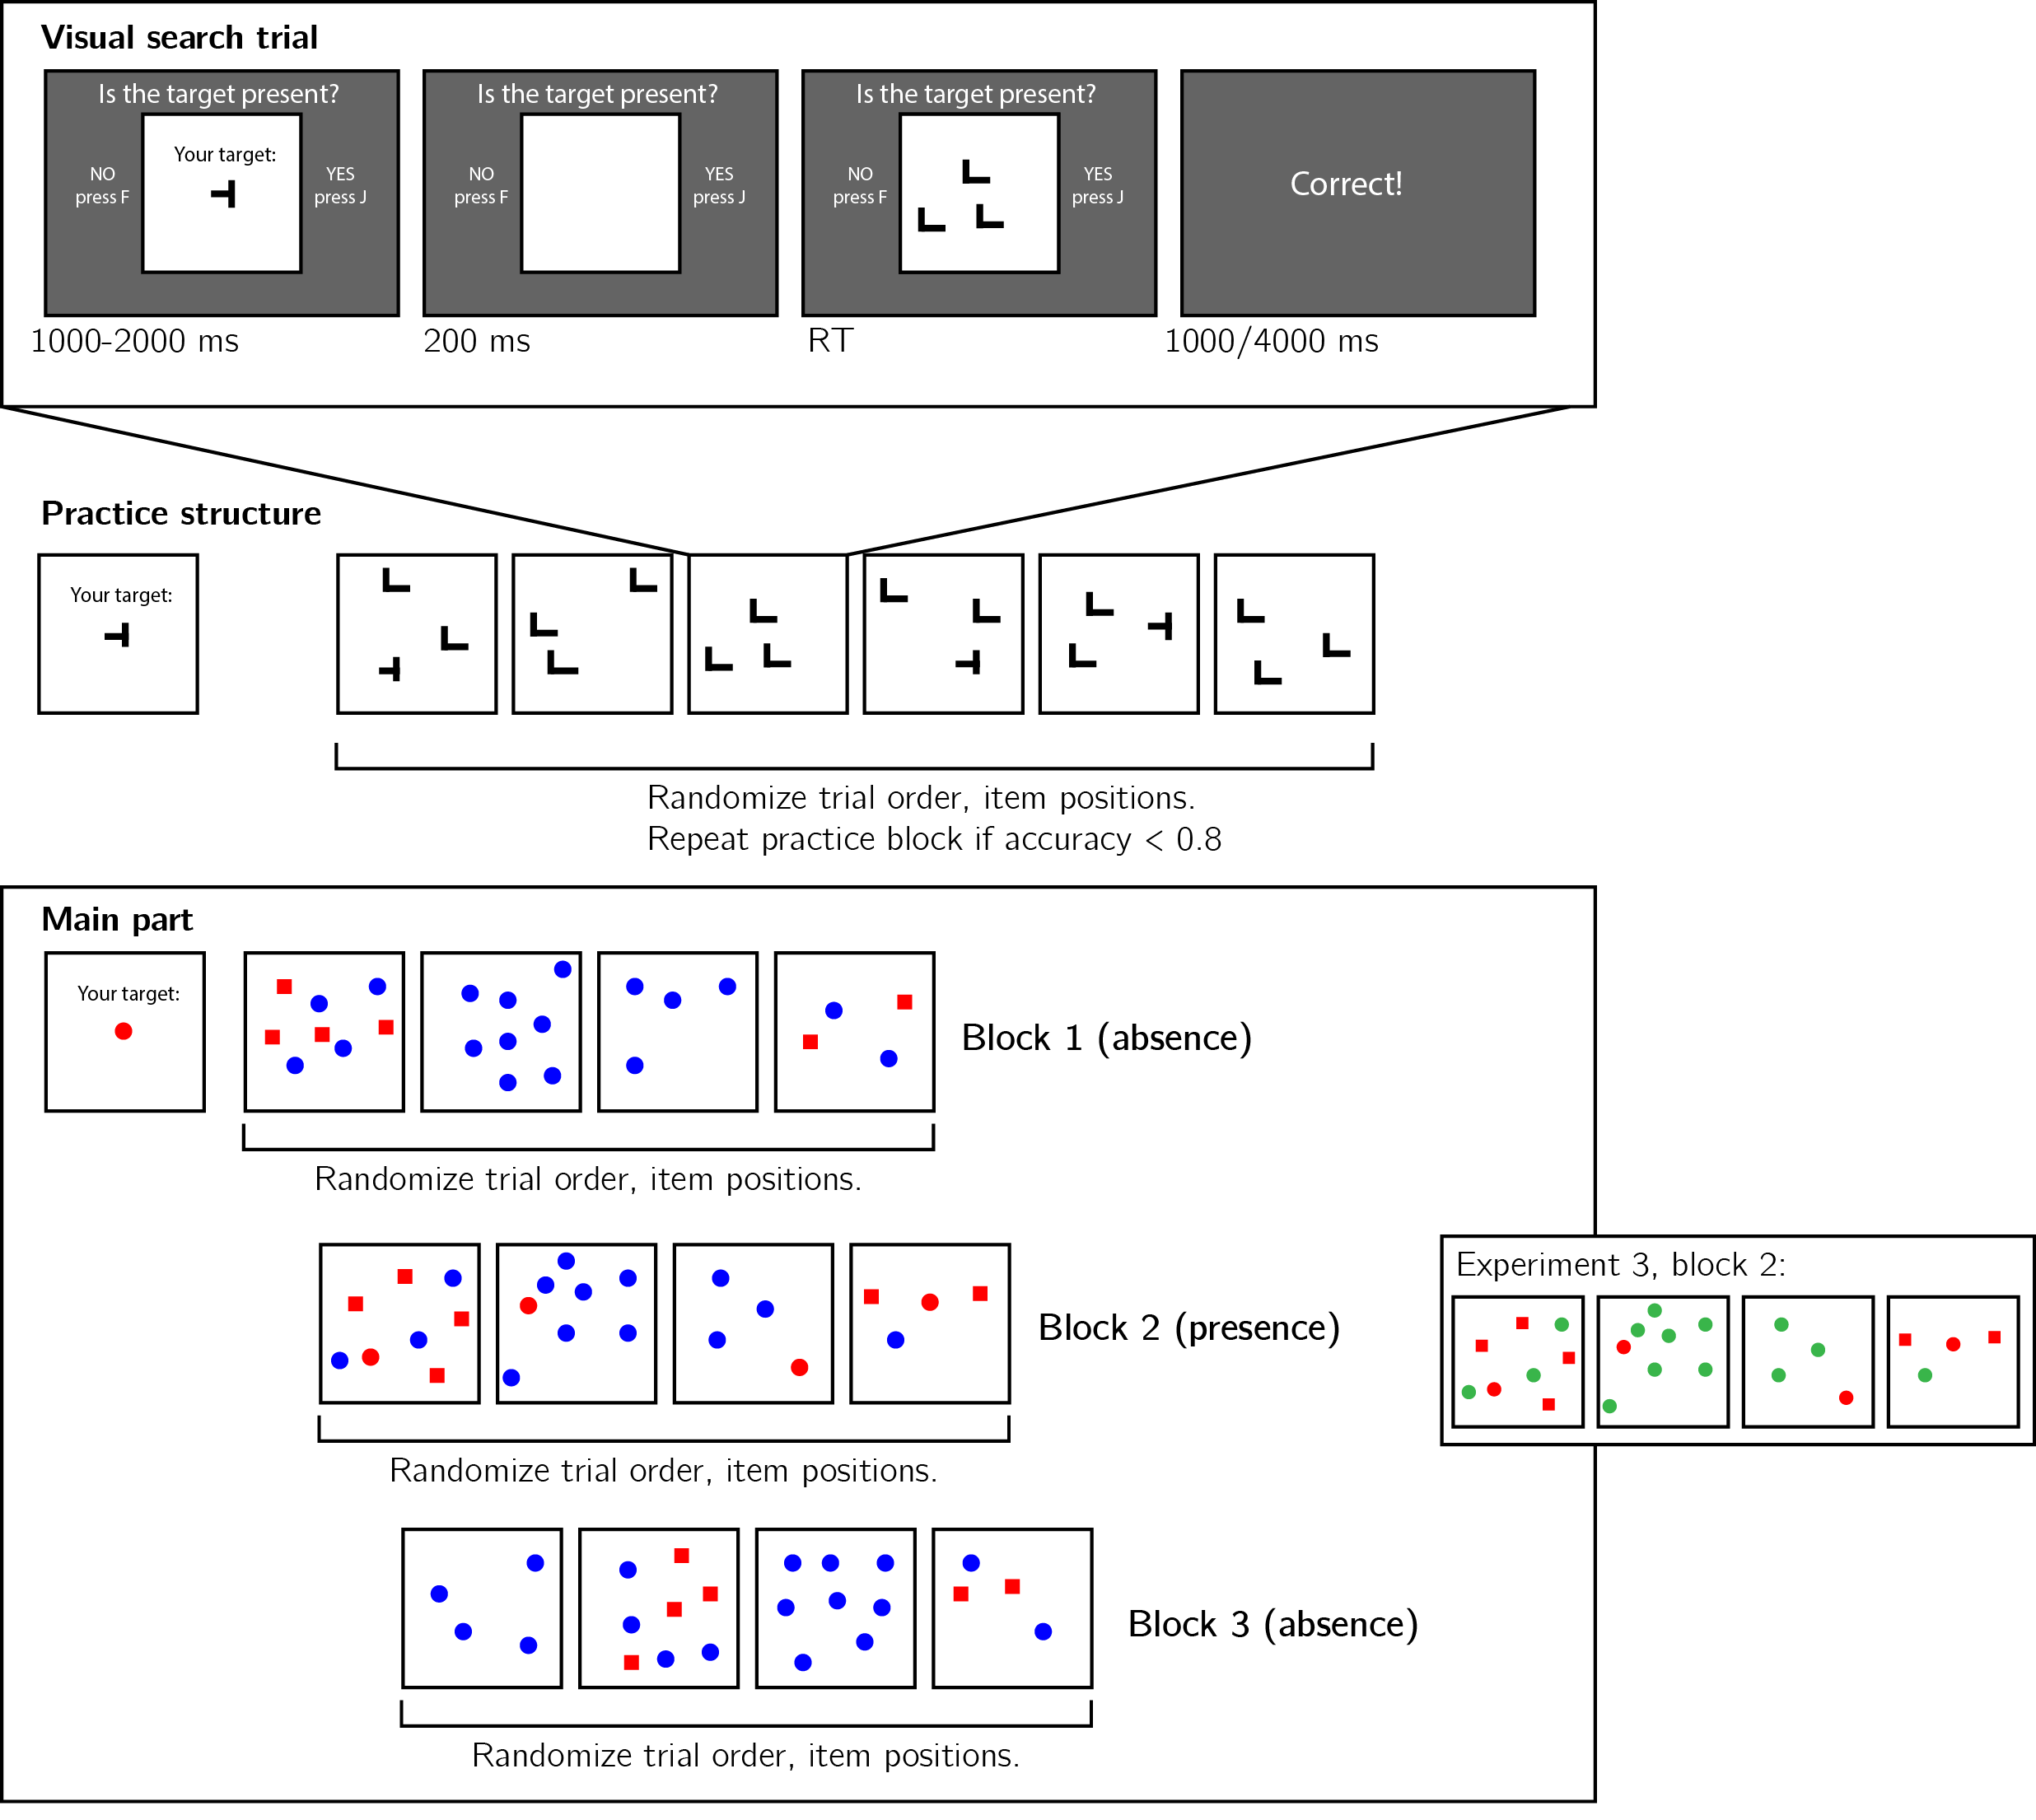
\includegraphics[width=1\linewidth]{figures/design} \caption{Design for experiments 1-3. Top panel: each visual search trial will start with a screen indicting the target stimulus. The search display will remain visible until a response is recorded. To motivate accurate responses, the feedback screen will remain visible for one second following correct responses and for four seconds following errors. Middle panel: after reading the instructions, participants will practice the visual search task in blocks of 6 trials, until they reach an accuracy level of 0.83. Bottom panel: the main part of the experiment will comprise 12 trials only, in which the target will be a red circle. Unbeknown the subjects, only trials 5-8 (Block 2) will be Target Present trials, and the remaining trials will be Target Absent trials. Each 4-trial block will follow a 2 by 2 design, with factors being set size (4 or 8) and distractor type (color or conjunction; blue circles only or blue circles and red squares, respectively). In experiment 2, Blocks 1 and 3 will comprise Target Present trials, and block 2 Target Absent trials. In block 2 of experiment 3, blue circles will be replaced with green circles.}\label{fig:design}
\end{figure}

In the main part of the experiment, participants will look for a red circle among blue circles or a mixed array of blue circles and red squares. Set sizes will be 4 or 12, resulting in a 2-by-2 design (search type: color or color\(\times\)shape, by set size: 4 or 12). Critically, and unknown to subjects, the first four trials will always be target-absent trials (one of each set-size \(\times\) search-type combination), presented in randomized order. These trials will be followed by the four corresponding target-present trials, presented in randomized order. The final four trials will again be target-absent trials, presented in randomized order.

\hypertarget{experiment-2-conditioned-on-experiment-1}{%
\subsection{Experiment 2 (conditioned on Experiment 1)}\label{experiment-2-conditioned-on-experiment-1}}

Experiment 2 will be identical to Experiment 1, except for the order of blocks. This experiment will start with 4 Target Presence trials, that will be followed by 4 Target Absent trials, followed by 4 Target Present trials. The purpose of this order reversal manipulation is to test whether the pattern observed in blocks 1 and 2 of Experiment 1 is unique to Target Absence trials, or alternatively emerges in the first trials of the experiment, regardless of the presence or absence of a target.

\hypertarget{experiment-3-conditioned-on-experiment-1}{%
\subsection{Experiment 3 (conditioned on Experiment 1)}\label{experiment-3-conditioned-on-experiment-1}}

Experiment 3 will be identical to Experiment 1, except for the four \enquote{Target Present} trials. Only in these four trials, blue circles will be replaced by green circles. The purpose of this manipulation is to test whether any learning between blocks 1 and 3 in Experiment 1 critically depends on direct experience with searching among distractors of a specific color, or alternatively, if learning about color search efficiency generalizes across colors.

\hypertarget{data-analysis}{%
\subsection{Data analysis}\label{data-analysis}}

\hypertarget{rejection-criteria}{%
\subsubsection{Rejection criteria}\label{rejection-criteria}}

Participants will be excluded for making more than one error in the main part of the experiment, or for having extremely fast or slow reaction times in one or more of the tasks (below 250 milliseconds or above 5 seconds in more than 25\% of the trials).

Error trials, and trials with response time below 250 milliseconds or above 1 second will be excluded from the response-time analysis.

\hypertarget{data-preprocessing}{%
\subsubsection{Data preprocessing}\label{data-preprocessing}}

To control for within-block trial order effects, a separate linear regression model will be fit to the data of each block, predicting search time as a function of trial serial order (\(RT \sim \beta_0+\beta_1i\), with \(i\) denoting the mean-centered serial position within a block). Search times will be corrected by subtracting the product of the slope and the mean-centered serial position, in a block-wise manner.

\hypertarget{hypotheses-and-analysis-plan}{%
\subsubsection{Hypotheses and analysis plan}\label{hypotheses-and-analysis-plan}}

Subject-wise search slopes will be extracted for each combination of search type (color or conjunction) and block number (first or third) by fitting a linear regression model to the reaction time data with one intercept and one set-size term.

Analysis for Experiments 1 and 3 will follow the same procedure: a positive control based on Target Present trials, a test of the presence of a pop-out effect for color search in block 1, and a test for the change in slope for color search between blocks 1 and 3. All hypotheses will be tested using a repeated-measures t-test, with a significance level of 0.05. Experiment 2 will be analyzed in a similar manner with some changes, indicated below.

Given the fact that we only have one trial per cell, one excluded trial is sufficient to make some hypotheses impossible to test on a given participant. For this reason, for each hypothesis separately, participants will be included only if all necessary trials meet our inclusion criteria. This means that some hypotheses may be tested on slightly different subsets of participants.

\emph{Hypothesis 1 (Positive control)}: To validate our methods and the quality of our data, we will test for a difference between search slopes for color and conjunction search in block 2 (Target Present). Based on previous work we expect a steeper slope for conjunction than for color search (Treisman \& Gelade, 1980; Wolfe, 1998). This positive control will serve to confirm that these effects are detectable in a large sample, even with only one trial per cell.

\emph{Hypothesis 2}: Pop-out for color absence in block 1. Throughout our analysis, we will define pop-out as a search slope significantly lower than 10 ms/item. This cutoff was chosen based on empirical distributions of search slopes in feature search (Wolfe, 1998). We will test the null hypothesis that the search slope in the color search, block 1 (Target Absent) equals to or is higher than 10ms/item, using a t-test. We will further test the null hypothesis that search slopes for color and conjunction searches in blocks 1 are equal.

\emph{Hypothesis 3}: Pop-out for color absence in block 3. We will test the null hypothesis that the search slope in the color search, block 3 (target absent) equals to or is higher than 10ms/item, using a t-test. We will further test the null hypothesis that search slopes for color and conjunction searches in blocks 3 are equal.

\emph{Hypothesis 4}: Search slope for color search changes between blocks 1 and 3. We will test the null hypothesis that the search slope in the color search, block 1 (target absent) equals to search slope in the color search, block 1 (target absent).

\emph{Hypothesis 5}: The change in search slopes between blocks 1 and 3 is different for color and for conjunction searches. To rule out a nonspecific change in search slope between blocks 1 and 3, We will compare the difference in search slopes for color search between block 1 and 3 with the difference in search slopes for conjunction search for the same blocks.

Experiments 2 will be run only if we find no pop out effect for color search in block 1 (Hypotheses 2). Analysis for Experiment 2 will be similar to analysis for Experiments 1 and 3, with the following changes: Hypothesis 1 (positive control) will be performed on block 3, Hypothesis 2 (pop out for color absence) will be performed on block 2, and Hypotheses 4 and 5 will test for changes in the slope for Target Present, rather than Target Absent trials.

Experiments 3 will be run only if we find a significant, non-generic learning effect between blocks 1 and 3 (Hypotheses 4 and 5).

Experiment 2 will test the specificity of the effect for Target-Absent trials, rather than Target Present trials more generally. Based on the idea that metacognitive knowledge is required for inference about absence much more than for inference about presence, we expect to find no learning effect between these blocks. Experiment 3 will test subjects' ability to generalize across different colors in learning from Target Present trials and in using this knowledge to guide their inference about absence in Target Absent trials.

\hypertarget{statistical-power}{%
\subsection{Statistical power}\label{statistical-power}}

Statistical power calculations were performed using the R-pwr package (Champely, 2020).

With a minimum of 200 participants for each hypothesis, we will have statistical power of 95\% to detect effect size of 200, 0.256140388328483, 0.05, 0.95, two.sided, n is number of \emph{pairs}, Paired t test power calculation in a two tailed test.

\newpage

\hypertarget{references}{%
\section{References}\label{references}}

\begingroup
\setlength{\parindent}{-0.5in}
\setlength{\leftskip}{0.5in}

\hypertarget{refs}{}
\leavevmode\hypertarget{ref-R-papaja}{}%
Aust, F., \& Barth, M. (2020). \emph{papaja: Create APA manuscripts with R Markdown}. Retrieved from \url{https://github.com/crsh/papaja}

\leavevmode\hypertarget{ref-R-Matrix}{}%
Bates, D., \& Maechler, M. (2019). \emph{Matrix: Sparse and dense matrix classes and methods}. Retrieved from \url{https://CRAN.R-project.org/package=Matrix}

\leavevmode\hypertarget{ref-R-brms_a}{}%
Bürkner, P.-C. (2017). brms: An R package for Bayesian multilevel models using Stan. \emph{Journal of Statistical Software}, \emph{80}(1), 1--28. \url{https://doi.org/10.18637/jss.v080.i01}

\leavevmode\hypertarget{ref-R-brms_b}{}%
Bürkner, P.-C. (2018). Advanced Bayesian multilevel modeling with the R package brms. \emph{The R Journal}, \emph{10}(1), 395--411. \url{https://doi.org/10.32614/RJ-2018-017}

\leavevmode\hypertarget{ref-R-pwr}{}%
Champely, S. (2020). \emph{Pwr: Basic functions for power analysis}. Retrieved from \url{https://CRAN.R-project.org/package=pwr}

\leavevmode\hypertarget{ref-chun1996just}{}%
Chun, M. M., \& Wolfe, J. M. (1996). Just say no: How are visual searches terminated when there is no target present? \emph{Cognitive Psychology}, \emph{30}(1), 39--78.

\leavevmode\hypertarget{ref-R-Rcpp_b}{}%
Eddelbuettel, D., \& Balamuta, J. J. (2017). Extending extitR with extitC++: A Brief Introduction to extitRcpp. \emph{PeerJ Preprints}, \emph{5}, e3188v1. \url{https://doi.org/10.7287/peerj.preprints.3188v1}

\leavevmode\hypertarget{ref-R-Rcpp_a}{}%
Eddelbuettel, D., \& François, R. (2011). Rcpp: Seamless R and C++ integration. \emph{Journal of Statistical Software}, \emph{40}(8), 1--18. \url{https://doi.org/10.18637/jss.v040.i08}

\leavevmode\hypertarget{ref-R-MESS}{}%
Ekstrøm, C. T. (2019). \emph{MESS: Miscellaneous esoteric statistical scripts}. Retrieved from \url{https://CRAN.R-project.org/package=MESS}

\leavevmode\hypertarget{ref-R-purrr}{}%
Henry, L., \& Wickham, H. (2020). \emph{Purrr: Functional programming tools}. Retrieved from \url{https://CRAN.R-project.org/package=purrr}

\leavevmode\hypertarget{ref-R-BayesFactor}{}%
Morey, R. D., \& Rouder, J. N. (2018). \emph{BayesFactor: Computation of bayes factors for common designs}. Retrieved from \url{https://CRAN.R-project.org/package=BayesFactor}

\leavevmode\hypertarget{ref-R-tibble}{}%
Müller, K., \& Wickham, H. (2020). \emph{Tibble: Simple data frames}. Retrieved from \url{https://CRAN.R-project.org/package=tibble}

\leavevmode\hypertarget{ref-R-lsr}{}%
Navarro, D. (2015). \emph{Learning statistics with r: A tutorial for psychology students and other beginners. (Version 0.5)}. Adelaide, Australia: University of Adelaide. Retrieved from \url{http://ua.edu.au/ccs/teaching/lsr}

\leavevmode\hypertarget{ref-R-coda}{}%
Plummer, M., Best, N., Cowles, K., \& Vines, K. (2006). CODA: Convergence diagnosis and output analysis for mcmc. \emph{R News}, \emph{6}(1), 7--11. Retrieved from \url{https://journal.r-project.org/archive/}

\leavevmode\hypertarget{ref-R-base}{}%
R Core Team. (2019). \emph{R: A language and environment for statistical computing}. Vienna, Austria: R Foundation for Statistical Computing. Retrieved from \url{https://www.R-project.org/}

\leavevmode\hypertarget{ref-R-broom}{}%
Robinson, D., \& Hayes, A. (2020). \emph{Broom: Convert statistical analysis objects into tidy tibbles}. Retrieved from \url{https://CRAN.R-project.org/package=broom}

\leavevmode\hypertarget{ref-treisman1980feature}{}%
Treisman, A. M., \& Gelade, G. (1980). A feature-integration theory of attention. \emph{Cognitive Psychology}, \emph{12}(1), 97--136.

\leavevmode\hypertarget{ref-R-ggplot2}{}%
Wickham, H. (2016). \emph{Ggplot2: Elegant graphics for data analysis}. Springer-Verlag New York. Retrieved from \url{https://ggplot2.tidyverse.org}

\leavevmode\hypertarget{ref-R-stringr}{}%
Wickham, H. (2019). \emph{Stringr: Simple, consistent wrappers for common string operations}. Retrieved from \url{https://CRAN.R-project.org/package=stringr}

\leavevmode\hypertarget{ref-R-forcats}{}%
Wickham, H. (2020). \emph{Forcats: Tools for working with categorical variables (factors)}. Retrieved from \url{https://CRAN.R-project.org/package=forcats}

\leavevmode\hypertarget{ref-R-tidyverse}{}%
Wickham, H., Averick, M., Bryan, J., Chang, W., McGowan, L. D., François, R., \ldots{} Yutani, H. (2019). Welcome to the tidyverse. \emph{Journal of Open Source Software}, \emph{4}(43), 1686. \url{https://doi.org/10.21105/joss.01686}

\leavevmode\hypertarget{ref-R-dplyr}{}%
Wickham, H., François, R., Henry, L., \& Müller, K. (2020). \emph{Dplyr: A grammar of data manipulation}. Retrieved from \url{https://CRAN.R-project.org/package=dplyr}

\leavevmode\hypertarget{ref-R-tidyr}{}%
Wickham, H., \& Henry, L. (2020). \emph{Tidyr: Tidy messy data}. Retrieved from \url{https://CRAN.R-project.org/package=tidyr}

\leavevmode\hypertarget{ref-R-readr}{}%
Wickham, H., Hester, J., \& Francois, R. (2018). \emph{Readr: Read rectangular text data}. Retrieved from \url{https://CRAN.R-project.org/package=readr}

\leavevmode\hypertarget{ref-R-cowplot}{}%
Wilke, C. O. (2019). \emph{Cowplot: Streamlined plot theme and plot annotations for 'ggplot2'}. Retrieved from \url{https://CRAN.R-project.org/package=cowplot}

\leavevmode\hypertarget{ref-wolfe1998can}{}%
Wolfe, J. M. (1998). What can 1 million trials tell us about visual search? \emph{Psychological Science}, \emph{9}(1), 33--39.

\endgroup

\newpage

\hypertarget{supplementary-information}{%
\section{Supplementary information}\label{supplementary-information}}

\hypertarget{pilot-data-and-analysis}{%
\section{Pilot data and analysis}\label{pilot-data-and-analysis}}

\hypertarget{pilot-experiment}{%
\subsection{Pilot Experiment}\label{pilot-experiment}}

We used R (Version 3.6.0; R Core Team, 2019) and the R-packages \emph{\}base} {[}@\}R-base{]}, \emph{\}reticulate} {[}@\}R-reticulate{]}, \emph{base} (Version 3.6.0; @\}R-base; R Core Team, 2019), \emph{BayesFactor} (Version 0.9.12.4.2; Morey \& Rouder, 2018), \emph{brms} (Version 2.13.0; Bürkner, 2017, 2018), \emph{broom} (Version 0.5.6; Robinson \& Hayes, 2020), \emph{coda} (Version 0.19.3; Plummer, Best, Cowles, \& Vines, 2006), \emph{cowplot} (Version 1.0.0; Wilke, 2019), \emph{dplyr} (Version 1.0.0; Wickham et al., 2020), \emph{forcats} (Version 0.5.0; Wickham, 2020), \emph{ggplot2} (Version 3.3.1; Wickham, 2016), \emph{lsr} (Version 0.5; Navarro, 2015), \emph{Matrix} (Version 1.2.17; Bates \& Maechler, 2019), \emph{MESS} (Version 0.5.6; Ekstrøm, 2019), \emph{papaja} (Version 0.1.0.9942; Aust \& Barth, 2020, 2020, 2020), \emph{purrr} (Version 0.3.4; Henry \& Wickham, 2020), \emph{pwr} (Version 1.3.0; Champely, 2020), \emph{Rcpp} (Version 1.0.4.6; Eddelbuettel \& François, 2011; Eddelbuettel \& Balamuta, 2017), \emph{readr} (Version 1.3.1; Wickham, Hester, \& Francois, 2018), \emph{stringr} (Version 1.4.0; Wickham, 2019), \emph{tibble} (Version 3.0.1; Müller \& Wickham, 2020), \emph{tidyr} (Version 1.1.0; Wickham \& Henry, 2020), and \emph{tidyverse} (Version 1.3.0; Wickham, Averick, et al., 2019) for all our analyses.

\hypertarget{participants-1}{%
\subsection{Participants}\label{participants-1}}

We collected data from a total of 181 participants, recruited on Prolific. The entire experiment took 3 minutes to complete (median completion time: 3:06 minutes). Participants were paid £0.38 for their participation, equivalent to an hourly wage of £7.6. The data of 163 participants met our inclusion criteria and were used for the main analysis.

\hypertarget{material}{%
\subsection{Material}\label{material}}

\hypertarget{procedure}{%
\subsection{Procedure}\label{procedure}}

The pilot task, as delivered to participants, can be accessed \href{http://167.99.93.4/publix/30/start?batchId=51\&generalMultiple}{in the following link}.
The pilot task followed the procedure for Experiment 1, described in the Methods section above.

\hypertarget{results}{%
\subsection{Results}\label{results}}

Overall mean accuracy was 0.95 (standard deviation =0.06). The median reaction time was 626.56 ms (median obsolute deviation = 129.59). In all further analysis, only correct trials with response time between 250 and 1000 ms were included.

\emph{Hypothesis 1 (positive control)}: Search times in block 2 (target-present) followed the expected pattern, with a steep slope for conjunction search (\(M = 14.97\), 95\% CI \([8.61\), \(21.34]\)) and a shallow slope for conjunction search (\(M = 5.26\), 95\% CI \([1.19\), \(9.33]\)). The slope for color search was significantly lower than 5 ms/item and thus met our criterion for being considered \enquote{pop-out} (\(t(138) = -2.30\), \(p = .011\)). Furthermore, the difference between the slopes was significant (\(t(105) = 2.90\), \(p = .005\)). This positive control served to validate our method.

\emph{Hypothesis 2}: Our central focus was on results from block 1 (target-absent). Here participants didn't yet have experience with searching for the red circle. Similar to the second block, the slope for the conjunction search was steep (\(M = 15.39\), 95\% CI \([5.99\), \(24.79]\)). However, in this first block the slope of the color search did not meet our criterion for being considered \enquote{pop-out} (\(M = 9.56\), 95\% CI \([-\infty\), \(16.12]\), \(t(116) = -0.11\), \(p = .456\)). Furthermore, search slope for color search in this first block was indistinguishable from that of the conjunction search (\(t(61) = 0.64\), \(p = .526\)), suggesting that some experience was needed in order for the color pop-out effect to manifest in target-absence searches.

\emph{Hypothesis 3}: Next, we tested the effect of experience on search slope. In the third block participants made \enquote{Target Absent} judgments, but in contrast to the first block here they already had experience with \enquote{Target Present} trials. In this third block, color search complied with our criterion for \enquote{pop-out} (\(M = -2.95\), 95\% CI \([-\infty\), \(1.51]\), \(t(136) = -4.81\), \(p < .001\)), and was significantly different from the search for conjunction search (\(t(106) = 7.28\), \(p < .001\)). In this third blocks, participants already showed a full pop-out effect for color search.

\emph{Hypothesis 4}: To quantify the learning effect for color search, we directly contrasted the search slope for color search in blocks 1 and 3. by contrasting the color slopes for the target-absence blocks 1 and 3. By the third block (or 9th trial), the slope for color search was already significantly different from the slope in block 1 (\(t(101) = 2.48\), \(p = .015\)), indicating a learning effect.

\emph{Hypothesis 5}: Finally, to make sure that this learning effect is not generic (for example, participants generally become more efficient in their searches), we quantified the interaction effect of search type (color, conjunction), and block number (1 and 3). This effect was only marginally significant in our sample (\(M = 18.48\), 95\% CI \([-1.76\), \(38.72]\), \(t(49) = 1.83\), \(p = .073\)).

\begin{figure}
\centering
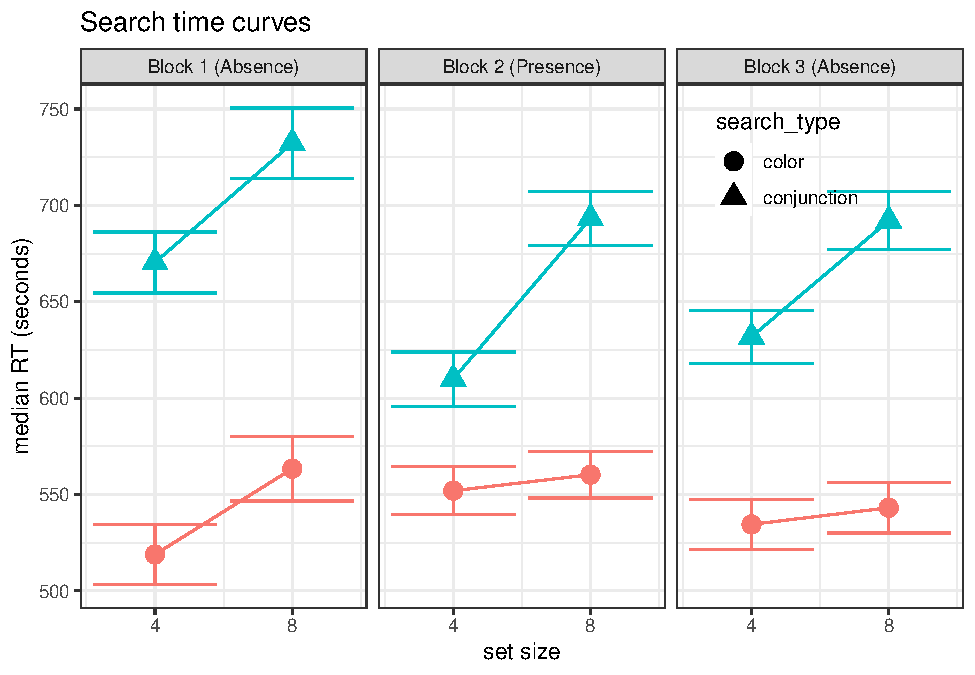
\includegraphics{termination_files/figure-latex/RT-pilot-1.pdf}
\caption{\label{fig:RT-pilot}Median search time by distractor set size for the two search tasks across the three blocks. Correct responses only. Error bars represent the standard error of the median.}
\end{figure}

\newpage

\hypertarget{references-1}{%
\section{References}\label{references-1}}

\begingroup
\setlength{\parindent}{-0.5in}
\setlength{\leftskip}{0.5in}

\hypertarget{refs}{}
\leavevmode\hypertarget{ref-R-papaja}{}%
Aust, F., \& Barth, M. (2020). \emph{papaja: Create APA manuscripts with R Markdown}. Retrieved from \url{https://github.com/crsh/papaja}

\leavevmode\hypertarget{ref-R-Matrix}{}%
Bates, D., \& Maechler, M. (2019). \emph{Matrix: Sparse and dense matrix classes and methods}. Retrieved from \url{https://CRAN.R-project.org/package=Matrix}

\leavevmode\hypertarget{ref-R-brms_a}{}%
Bürkner, P.-C. (2017). brms: An R package for Bayesian multilevel models using Stan. \emph{Journal of Statistical Software}, \emph{80}(1), 1--28. \url{https://doi.org/10.18637/jss.v080.i01}

\leavevmode\hypertarget{ref-R-brms_b}{}%
Bürkner, P.-C. (2018). Advanced Bayesian multilevel modeling with the R package brms. \emph{The R Journal}, \emph{10}(1), 395--411. \url{https://doi.org/10.32614/RJ-2018-017}

\leavevmode\hypertarget{ref-R-pwr}{}%
Champely, S. (2020). \emph{Pwr: Basic functions for power analysis}. Retrieved from \url{https://CRAN.R-project.org/package=pwr}

\leavevmode\hypertarget{ref-chun1996just}{}%
Chun, M. M., \& Wolfe, J. M. (1996). Just say no: How are visual searches terminated when there is no target present? \emph{Cognitive Psychology}, \emph{30}(1), 39--78.

\leavevmode\hypertarget{ref-R-Rcpp_b}{}%
Eddelbuettel, D., \& Balamuta, J. J. (2017). Extending extitR with extitC++: A Brief Introduction to extitRcpp. \emph{PeerJ Preprints}, \emph{5}, e3188v1. \url{https://doi.org/10.7287/peerj.preprints.3188v1}

\leavevmode\hypertarget{ref-R-Rcpp_a}{}%
Eddelbuettel, D., \& François, R. (2011). Rcpp: Seamless R and C++ integration. \emph{Journal of Statistical Software}, \emph{40}(8), 1--18. \url{https://doi.org/10.18637/jss.v040.i08}

\leavevmode\hypertarget{ref-R-MESS}{}%
Ekstrøm, C. T. (2019). \emph{MESS: Miscellaneous esoteric statistical scripts}. Retrieved from \url{https://CRAN.R-project.org/package=MESS}

\leavevmode\hypertarget{ref-R-purrr}{}%
Henry, L., \& Wickham, H. (2020). \emph{Purrr: Functional programming tools}. Retrieved from \url{https://CRAN.R-project.org/package=purrr}

\leavevmode\hypertarget{ref-R-BayesFactor}{}%
Morey, R. D., \& Rouder, J. N. (2018). \emph{BayesFactor: Computation of bayes factors for common designs}. Retrieved from \url{https://CRAN.R-project.org/package=BayesFactor}

\leavevmode\hypertarget{ref-R-tibble}{}%
Müller, K., \& Wickham, H. (2020). \emph{Tibble: Simple data frames}. Retrieved from \url{https://CRAN.R-project.org/package=tibble}

\leavevmode\hypertarget{ref-R-lsr}{}%
Navarro, D. (2015). \emph{Learning statistics with r: A tutorial for psychology students and other beginners. (Version 0.5)}. Adelaide, Australia: University of Adelaide. Retrieved from \url{http://ua.edu.au/ccs/teaching/lsr}

\leavevmode\hypertarget{ref-R-coda}{}%
Plummer, M., Best, N., Cowles, K., \& Vines, K. (2006). CODA: Convergence diagnosis and output analysis for mcmc. \emph{R News}, \emph{6}(1), 7--11. Retrieved from \url{https://journal.r-project.org/archive/}

\leavevmode\hypertarget{ref-R-base}{}%
R Core Team. (2019). \emph{R: A language and environment for statistical computing}. Vienna, Austria: R Foundation for Statistical Computing. Retrieved from \url{https://www.R-project.org/}

\leavevmode\hypertarget{ref-R-broom}{}%
Robinson, D., \& Hayes, A. (2020). \emph{Broom: Convert statistical analysis objects into tidy tibbles}. Retrieved from \url{https://CRAN.R-project.org/package=broom}

\leavevmode\hypertarget{ref-treisman1980feature}{}%
Treisman, A. M., \& Gelade, G. (1980). A feature-integration theory of attention. \emph{Cognitive Psychology}, \emph{12}(1), 97--136.

\leavevmode\hypertarget{ref-R-ggplot2}{}%
Wickham, H. (2016). \emph{Ggplot2: Elegant graphics for data analysis}. Springer-Verlag New York. Retrieved from \url{https://ggplot2.tidyverse.org}

\leavevmode\hypertarget{ref-R-stringr}{}%
Wickham, H. (2019). \emph{Stringr: Simple, consistent wrappers for common string operations}. Retrieved from \url{https://CRAN.R-project.org/package=stringr}

\leavevmode\hypertarget{ref-R-forcats}{}%
Wickham, H. (2020). \emph{Forcats: Tools for working with categorical variables (factors)}. Retrieved from \url{https://CRAN.R-project.org/package=forcats}

\leavevmode\hypertarget{ref-R-tidyverse}{}%
Wickham, H., Averick, M., Bryan, J., Chang, W., McGowan, L. D., François, R., \ldots{} Yutani, H. (2019). Welcome to the tidyverse. \emph{Journal of Open Source Software}, \emph{4}(43), 1686. \url{https://doi.org/10.21105/joss.01686}

\leavevmode\hypertarget{ref-R-dplyr}{}%
Wickham, H., François, R., Henry, L., \& Müller, K. (2020). \emph{Dplyr: A grammar of data manipulation}. Retrieved from \url{https://CRAN.R-project.org/package=dplyr}

\leavevmode\hypertarget{ref-R-tidyr}{}%
Wickham, H., \& Henry, L. (2020). \emph{Tidyr: Tidy messy data}. Retrieved from \url{https://CRAN.R-project.org/package=tidyr}

\leavevmode\hypertarget{ref-R-readr}{}%
Wickham, H., Hester, J., \& Francois, R. (2018). \emph{Readr: Read rectangular text data}. Retrieved from \url{https://CRAN.R-project.org/package=readr}

\leavevmode\hypertarget{ref-R-cowplot}{}%
Wilke, C. O. (2019). \emph{Cowplot: Streamlined plot theme and plot annotations for 'ggplot2'}. Retrieved from \url{https://CRAN.R-project.org/package=cowplot}

\leavevmode\hypertarget{ref-wolfe1998can}{}%
Wolfe, J. M. (1998). What can 1 million trials tell us about visual search? \emph{Psychological Science}, \emph{9}(1), 33--39.

\endgroup

\end{document}
